%  PHDTHESIS TEMPLATE FILE
%  Adopted from Thomas Fabricius and Henrik Aalborg Nielsen
%  Jan Larsen, IMM, DTU, Nov 2003 ver 1.0
%  Updated by Finn Kuno Christensen, fkc@imm.dtu.dk Aug 15, 2008

%  COMPILATION STEPS USING INVOLVING A PS FILE
%\documentclass[10pt,twoside,dvips]{book}
%  latex phdthesis.tex
%  dvips -D600 -Pamz -Pcmz -j0 phdthesis.dvi -o phdthesis.ps
%  ps2pdf -sPAPERSIZE=b5 phdthesis.ps phdthesis.pdf (or use Acrobat Distiller)

%  COMPILATION STEP USING PDFLATEX
\documentclass[11pt,twoside]{book}
%  pdflatex phdthesis.tex

\usepackage[utf8]{inputenc}
\usepackage{url}
\usepackage{python}
\usepackage[round]{natbib}
\usepackage{color}
\usepackage{caption}
\captionsetup{font={small,it},labelfont=bf}
\usepackage{subfig}
\usepackage{paralist}
\definecolor{mygray}{RGB}{244,244,244}
\definecolor{gray}{gray}{0.5}
\definecolor{myredish}{RGB}{193,33,97}
\definecolor{grayblue}{RGB}{91,112,142}
\definecolor{myorange}{RGB}{255,134,0}
\definecolor{green}{rgb}{0,0.4,0}
\usepackage{tabularx}

\usepackage[pdftex]{hyperref}
\hypersetup{ 
    colorlinks,% 
    citecolor=grayblue,% 
    filecolor=grayblue,% 
    linkcolor=grayblue,% 
    urlcolor=grayblue 
}

\newcommand\mydef[1]{\emph{#1}}
\newcommand\mytodo[1]{\textbf{\textcolor{red}{TODO: #1}}}
\newcommand\fn[1]{{\ttfamily\small #1}}
\newcolumntype{R}{>{\raggedleft\arraybackslash}X}%
\newcommand\appref[1]{appendix \ref{app:#1}}
\newcommand\mypagebreak{\vspace{\stretch{1}}\pagebreak}
\newcommand\githuburl[1]{\url{https://github.com/alphabits/ford_challenge/tree/master/#1}}
\newcommand\norm[1]{||\,#1\,||}
\newcommand\ve[1]{\boldsymbol{#1}}
\newcommand\varop[1]{\text{Var}\,[#1]}
\newcommand\expop[1]{\text{E}\,[#1]}
\newcommand\covop[1]{\text{Cov}\,[#1]}
\newcommand\myimp{\quad\quad\Leftrightarrow}

\usepackage{lmodern}
\usepackage{fouriernc}
\usepackage[scaled]{beramono}
\usepackage{listings}
\lstset {                 % A rudimentary config that shows off some features.
    language=Python,
    basicstyle=\scriptsize\ttfamily, % Without beramono, we'd get cmtt, the teletype font.
    commentstyle=\textit, % cmtt doesn't do italics. It might do slanted text though.
    keywordstyle=\bfseries,
    framextopmargin=4pt,
    framexbottommargin=4pt,
    framexleftmargin=4pt,
    framexrightmargin=4pt,
    xleftmargin=4pt,
    xrightmargin=4pt,
    backgroundcolor=\color{mygray},
    frame=single,
    showstringspaces=false,
    captionpos=b,
    tabsize=4            % Or whatever you use in your editor, I suppose.
}

\renewcommand{\lstlistlistingname}{Code Listings}
\renewcommand{\lstlistingname}{Code Listing}

\lstset{
    language=python,
    stringstyle=\color{myorange},
    showstringspaces=false,
    alsoletter={1234567890},
    otherkeywords={\ , \}, \{},
    keywordstyle=\color{blue},
    emph={access,and,break,class,continue,def,del,elif ,else,%
    except,exec,finally,for,from,global,if,import,in,i s,%
    lambda,not,or,pass,print,raise,return,try,while},
    emphstyle=\color{myredish}\bfseries,
    emph={[2]True, False, None, self, __file__},
    emphstyle=[2]\color{green},
    emph={[3]from, import, as},
    emphstyle=[3]\color{blue},
    upquote=true,
    morecomment=[s]{"""}{"""},
    commentstyle=\color{gray}\slshape,
    emph={[4]1, 2, 3, 4, 5, 6, 7, 8, 9, 0},
    emphstyle=[4]\color{blue},
    literate=*{:}{{\textcolor{blue}:}}{1}%
    {=}{{\textcolor{blue}=}}{1}%
    {-}{{\textcolor{blue}-}}{1}%
    {+}{{\textcolor{blue}+}}{1}%
    {*}{{\textcolor{blue}*}}{1}%
    {!}{{\textcolor{blue}!}}{1}%
    {(}{{\textcolor{blue}(}}{1}%
    {)}{{\textcolor{blue})}}{1}%
    {[}{{\textcolor{blue}[}}{1}%
    {]}{{\textcolor{blue}]}}{1}%
    {<}{{\textcolor{blue}<}}{1}%
    {>}{{\textcolor{blue}>}}{1},%
    rulesepcolor=\color{blue}
}



%% Define a new 'leo' style for the url package that will use a smaller font.
\makeatletter
\def\url@leostyle{%
  \@ifundefined{selectfont}{\def\UrlFont{\sf}}{\def\UrlFont{\small\ttfamily}}}
\makeatother
%% Now actually use the newly defined style.
\urlstyle{leo}


%%%%%%%%%%% MODIFY THESE LINES ONLY %%%%%%%%%%%%%%%%%%%%%%%%%%%%%%%%%%%%%%%%%%%%%%%%%%%%%%%%%
\def\thesisyear{2011} % Year thesis submitted
\def\thesisnumber{70}  % Only number no year
\def\thesisauthor{Anders Hørsted} % Thesis author
\def\thesistitle{Detection of human alertness using supervised learning} % Title of thesis
\def\thesiskeywords{mathematical modelling}
\def\thesisISBN{} %OBSOBS provide ISBN number for industrial phd students ONLY
\def\thesisversion{print} %OBSOBS choose this for printed version send to printing
%\def\thesisversion{net} %OBSOBS choose this for the net version for the web and publication database
%%%%%%%%%%%%%%%%%%%%%%%%%%%%%%%%%%%%%%%%%%%%%%%%%%%%%%%%%%%%%%%%%%%%%%%%%%%%%%%%%%%%%%%%%%%%%

%%%%%%%%%%%%%%% DO NOT MODIFY START %%%%%%%%%%%%%%%%%%%%%%%%%%%%%%%%%%%%%%%%%%
\def\thesisISSN{0909-3192}
\def\ttitle{{\sf\textbf{\thesistitle}}}
\def\thesisdef{IMM-PHD-\thesisyear-\thesisnumber}
\usepackage{hyperref}
\def\printversion{print}
\ifx\thesisversion\printversion
  \special{papersize=176mm,250mm}
  \hypersetup{pdftitle={\thesistitle},
              pdfauthor={\thesisauthor},
              pdfsubject={\thesisdef},
              pdfkeywords={\thesiskeywords},
              breaklinks,
              bookmarksopen,
              bookmarksnumbered}
\else
  \hypersetup{pdftitle={\thesistitle},
              pdfauthor={\thesisauthor},
              pdfsubject={\thesisdef},
              pdfkeywords={\thesiskeywords},
              colorlinks,
              linkcolor=blue,
              breaklinks,
              bookmarksopen,
              bookmarksnumbered}
\fi


%%%%%%%%%%%%%% DO NOT MODIFY BELLOW START%%%%%%%%%%%%
\usepackage[english]{babel}
\usepackage{fancyheadings}
\usepackage{amsmath,amssymb,latexsym,epic,eepic,epsfig,graphics,psfrag}
\usepackage{theorem}
\usepackage{immthesislayout}

\newcommand{\papertitle}{}
\setcounter{tocdepth}{10} % 1 in final version 10 for debugging
\setcounter{secnumdepth}{3} % subsubsections get a number when this is 3

% PDF:
%\usepackage[pdftitle={PARAMETRIC AND NON-PARAMETRIC SYSTEM MODELLING},
%            pdfauthor={Henrik Aalborg Nielsen, IMM, DTU},
%            breaklinks,
%            bookmarksopen,
%            bookmarksnumbered]{hyperref}
%\hypersetup{pdftitle={\ttitle},
%%            pdfsubject={\thesisdef},
%            pdfkeywords={\thesiskeywords},
%            breaklinks,
%            bookmarksopen,
%            bookmarksnumbered}

\begin{document}
\thispagestyle{empty}
\vspace*{\fill}
\begin{center}
{\huge\ttitle}\\*[2.5cm]
\Large\sf\thesisauthor\\*[4.5cm]
\small\sf Kongens Lyngby \thesisyear\\
\small\sf IMM%-PHD-\thesisyear-\thesisnumber
\end{center}
\vspace*{\fill}
\newpage
\thispagestyle{empty}
\vspace*{11cm}
{\sf Technical University of Denmark}\\
{\sf Informatics and Mathematical Modelling}\\
{\sf Building 321, DK-2800 Kongens Lyngby, Denmark}\\
{\sf Phone +45 45253351, Fax +45 45882673}\\
{\sf reception@imm.dtu.dk}\\
{\sf www.imm.dtu.dk}

%\vspace*{2.5cm}
%\def\empty{}
%\ifx\thesisISBN\empty
%  {\sf IMM-PHD: ISSN \thesisISSN}
%\else
%  {\sf IMM-PHD: ISSN \thesisISSN, ISBN \thesisISBN}
%\fi


\frontmatter
\pagenumbering{roman}

%%%%%%%%%%%%%%% DO NOT MODIFY END %%%%%%%%%%%%%%%%%%%%%%%%%%%%%%%%%%%%%%%%%%%%



%%%%%%%PREFACE CHAPTERS INCLUDE%%%%%%%%%%%%%%%%%%%%%%%%%%%%%%%%%%%%%%%%%%%%%%

\chapter*{Summary}

This is the summary/abstract

\markboth{}{}
\chapter*{Resum\'e} %{Sammenfatning (Summary in Danish)}

På dansk

\markboth{}{}
\chapter*{Preface}

This project is the result of attending the course ``01666 Project work - Bachelor of Mathematics and Technology'' at the Technical University of Denmark. The course is mandatory for all Bachelors at Mathematics and Technology and counts for 10 ECTS points. \par

The subject of the project is held within the discipline called machine learning that, depending on how it is defined, can be seen as part of artificial intelligence or applied statistics. \par

The target group of the report is any student that have completed the course ``01005 Mathematics 1'' at DTU or a similar course at another university.

All files used in this project are available at \githuburl{ }.

\vspace{20mm}
Anders Hørsted \\
Christianshavn, June 2011

\markboth{}{}
\chapter*{Acknowledgements}

I thank my...

\markboth{}{}

%%%%%%%PREFACE CHAPTERS INCLUDE%%%%%%%%%%%%%%%%%%%%%%%%%%%%%%%%%%%%%%%%%%%%%%


\newpage\mbox{}\newpage
\chaptermark{Contents}
\renewcommand{\sectionmark}[1]{\markright{#1}}
\sectionmark{Contents}
\addtolength{\parskip}{-\baselineskip}
\tableofcontents
\addtolength{\parskip}{\baselineskip}
\renewcommand{\sectionmark}[1]{\markright{\thesection\ #1}}

\mainmatter
% Chapter 1, 2, ...
%%%%%%%MAIN CHAPTERS INCLUDE%%%%%%%%%%%%%%%%%%%%%%%%%%%%%%%%%%%%%%%%%%%%%%

\part{Introduction and data exploration}
\chapter{Introduction}
Igennem de sidste 30 år er computerens ydeevne vokset markant. Den forbedrede ydeevne har givet mulighed for at udføre statistisk dataanalyse, i et omfang der ikke tidligere har været muligt. En af de ting der er blevet mulighed for, er at programmere såkaldte "classifiers". Et godt eksempel på en classifier, er de programmer bankerne bruger til at opdage evt. snyd med kreditkort. Baseret på alle tidligere korttransaktioner, og viden om hvilke der var "falske"\ transaktioner, kan bankerne programmere en classifier, der med høj præcision kan forudsige om en ny transaktion er snyd eller ej. \\
Denne opgave tager udgangspunkt i en konkurrence på hjemmesiden kaggle.com. Konkurrencen er udbudt af Ford Motors og handler om at udvikle en classifier, der kan forudsige om en bilist er ved at blive ukoncentreret, mens han/hun kører bil. Til at udvikle denne classifier har Ford foretaget en række målinger på bilister, mens de kørte bil, og til hver måling er det blevet noteret om bilisten var opmærksom eller ej. Med udgangspunkt i disse målinger udarbejdes -- ved brug af de mest gængse metoder -- en række classifiers, og deres evne til at klassificere ny data sammenlignes.

\section{The competition} % (fold)
\label{sec:The competition}

% section The competition (end)

\subsection{Problemformulering}
I denne opgave vil jeg...
\begin{itemize}
    \item ... bruge de mest gængse klassifikationsmodeller (nearest neighbour, logistic regression, neural networks og SVM) til at lave en classifier der (forhåbentlig) kan forudsige om en bilist er ved at falde i søvn.
    \item ... undersøge hvor stor indflydelse den indledende databehandling (feature selection og outlier removal) har på det endelige resultat.
    \item ... undersøge om classifieren kan forbedres ved at implementere en Hidden Markov Model, der tager hensyn til det temporale aspekt af data.
    \item ... implementere en ensemble classifier, der kombinerer resultatet af flere classifiers i én classifier.
\end{itemize}

\mytodo{Remeber to define the different datasets}

\chapter{The Ford Challenge} 
In this chapter, the Ford competition that is the basis for this report, is introduced. Before introducing the Ford Challenge, a short overview of other online machine learning competitions is given. As part of introducing the Ford competition, the kaggle.com website that hosted the competition is presented, and the data set used in the competition is described in detail. But as metioned the chapter starts with a short overview of other online machine learning competitions.

\section{Other online machine learning competitions}
To get a little perspective on the Ford Challenge, this section gives a short review of some past and present online machine learning competitions.

\subsection[The Netflix Prize]{The Netflix Prize\protect\footnote{The section about The Netflix Prize is based on \citet{wiki:netflix_prize} and \citet{netflix_leaderboard}}}
One of the most talked about competitions, may very well be the Netflix Prize. The Netflix competition was launched on October 2, 2006 and the aim of the competition was to predict how users would grade new movies, based on a large dataset of previous grades. Why did the Netflix Prize gather a lot of attention? First of all the grand prize was \$1M, which is a lot of money. And secondly the dataset was huge, consisting of 100,480,507 ratings given by 480,189 users, leaving room for a lot of interesting new techniques to be tested. \par 
When the Netflix Prize was awarded on September 18, 2009, 5169 different teams had participated in the competition. The winning team consisted of three different teams that at one point decided to team-up and compete as a joint-team.\par 
Netflix originally wished to follow up the Netflix Prize, with another competition but decided to dismiss the idea, due to a lawsuit regarding privacy concerns related to the first Netflix Prize.

\subsection{KDD Cup}
Although the Netflix Prize gathered a lot of attention, it wasn't the first online machine learning competition. An example of an earlier competition is the KDD Cup. The KDD Cup started back in 1997 and is held every year. The subject changes every year, and can be anything from mining purchase data from an online store, to computer aided detection of breast cancer (the 2000 and 2008 competitions respectively).\par
This year the KDD Cup is held in cooporation with Yahoo! Labs and the task is to predict user ratings of musical items (both tracks, albums, artists and genres). One noteworthy detail about the 2011 KDD Cup is the huge data set, containing over 300 million ratings of more than 600,000 distinct items. \footnote{Read more about the KDD Cup history at \citet{kdd_cup_center}. For more info about the 2011 competition see \citet{kdd_cup_2011}}

\subsection{And many others}
The Netflix Prize and the KDD Cup are just two examples of online machine learning competitions. Many others exists, such as
\begin{itemize}
    \item \emph{The Hearst Challenge 2011} - Every year The Hearst Corporation hosts a machine learning competition. This year the task is to data mine the history of 1.8 million emails sent to subscribers of Hearst's publications, and then predict who will open emails in the future. \\
        Read more at \url{http://www.hearstchallenge.com}
    \item \emph{The Reclab Prize} - RichRelevance is a company that specializes in online product recommendation. They offer a \$1M prize for the team that first improves their product recommendation algorithm by 10\%. \\
        Read more at \url{http://www.overstockreclabprize.com}
    \item \emph{The Heritage Health Prize} - In this competition a dataset of anonymized patient data should be used to create a classifier that predicts and prevents unnecessary hospitalizations. With a first prize of \$3M, and the ethical issues surrounding the use of machine learning on patient data, this competition has received much attention.  \\
        Read more at \url{http://www.heritagehealthprize.com/}
\end{itemize}
Since almost all the machine learning competition websites needs the same functionality, websites that specializes in hosting competitions has appeared. One example of such a website is the kaggle.com website, which hosts The Ford Challenge.

\section{Kaggle.com and The Ford Challenge}
The first competition hosted by kaggle.com was started in April 2010, and since then a total of 18 competitions have been held. Every competition at kaggle.com has some background information, links to the data sets, a submission system and a forum, as seen in figure \ref{fig:fordchallenge_frontpage}. \par

\begin{figure}[tbhHp]
    \centering
        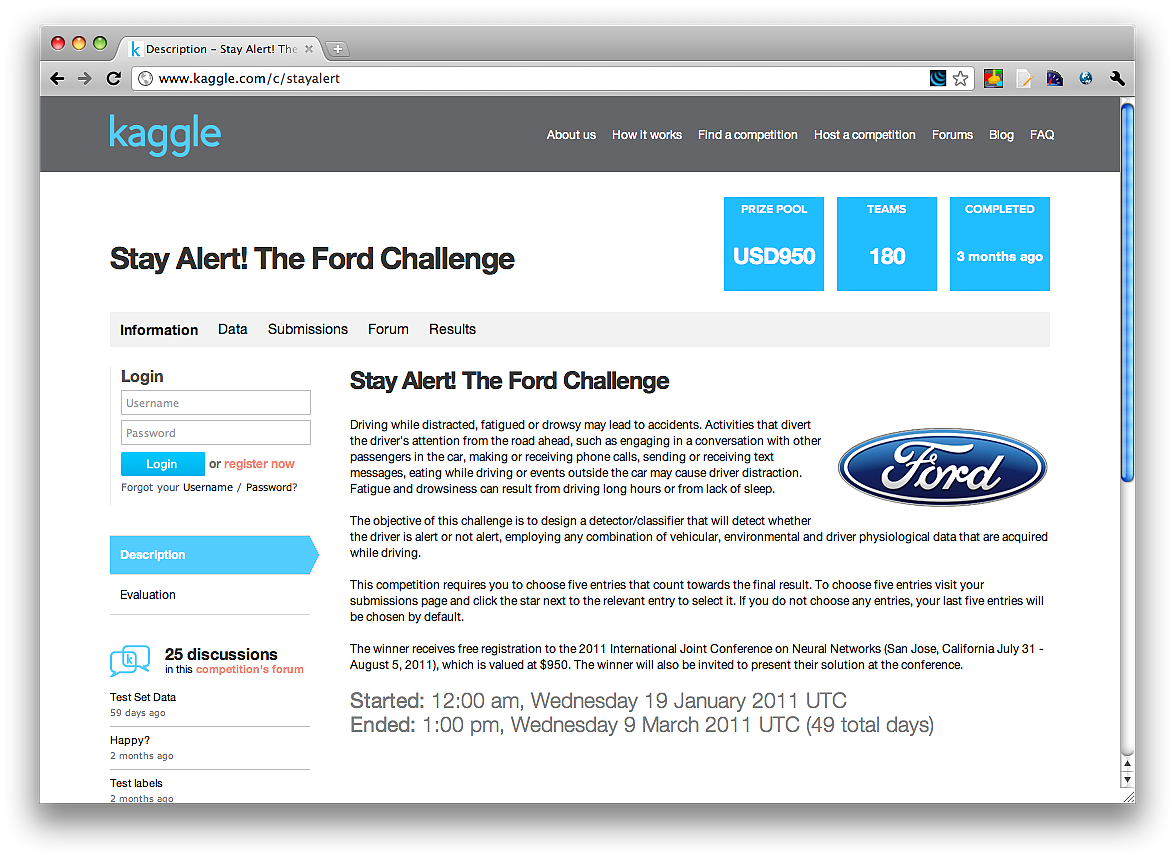
\includegraphics[width=.9\textwidth]{media/fordchallenge_frontpage.png}
    \caption{The Ford Challenge front page at the kaggle.com website}
    \label{fig:fordchallenge_frontpage}
\end{figure}

The Ford Challenge began on January 19, 2011. The task was to create a classifier that is able to detect when a driver is about to get distracted while driving. The dataset that Ford made available for the competition consisted of measurements of 30 different features, measured on drivers, along with a binary feature (IsAlert) that was 1 if the driver was alert and 0 otherwise. The 30 features was a mix of environmental, driver physiological and vehicular features\footnote{The dataset is explained in much more detail in the section \ref{sec:the-competition:dataset}}. Based on this dataset a classifier should be made, that predicts the IsAlert feature of a distinct test dataset held by Ford. \par
One detail that made the competition slightly different than many other competitions, was that Ford would not disclose any information about what the different features represented\footnote{See forum replies from the Ford spokesperson \citep{kaggle_forum_266,kaggle_forum_317}}. The official reason was that 
\begin{quote}
    ``We like to encourage the participants to pursue classification without preconceived notions based on prior knowledge of the subject, focusing on variables which lead them (based on their own experiments) to better classification." \citep{kaggle_forum_268_reply_2}
\end{quote}
Doubts about the true motive behind the lack of details about the features, was expressed by, what later turned out to be, the winner of the competition \citep{kaggle_forum_295_reply_3} \par

The performance of the classifiers was measured by calculating the AUC score (see section \ref{sec:auc}) of the classifiers, on the test set. A limit of two submissions per contestant was set as a way to counteract the possibility of someone reverse-engineering the IsAlert-feature of the test dataset. This could of cause be circumvented by one person registering more than once. And this was exactly what happened. On March 9, 2011 when the competition ended, two users had achieved exactly the same AUC (six significant digits) and other contestants immediately questioned the probability of two unrelated users getting exactly the same AUC \citep{kaggle_forum_327_reply_1}. One of the two leaders (Rosanne/Shen) quickly admitted that he and his friend had indeed used two accounts to get 4 submission per day \citep{kaggle_forum_327_reply_4}, and after some discussion in the forum, the leaders were disqualified. The end result was that the user Inference in third position was declared the official winner of the competition. \par

Two weeks after the competition ended, Inference described the technique used to win the competition. This will be described in detail in chapter \ref{sec:recreating}.

\subsection{The dataset}\label{sec:the-competition:dataset}
\begin{table}
    {\small\sffamily
    \begin{tabularx}{\textwidth}{ | l l l R R R R R R R R R | }
        \hline
        TrialID & ObsNum & IsAlert & P1 & $\dots$ & P8 & E1 & $\dots$ & E11 & V1 & $\dots$ & V11 \\\hline
        0 & 0 & 0 & 12.2 & $\dots$ & 1.2 & 4.3 & $\dots$ & 33 & 12 & $\dots$ & 7.34 \\
        $\vdots$ & & & & & & & & & & &$\vdots$ \\
        0 & 1200 & 1 & 11.1 & $\dots$ & 10.7 & 1.3 & $\dots$ & 21 & 8 & $\dots$ & 8.82 \\
        $\vdots$ & & & & & & & & & & &$\vdots$ \\
        510 & 1198 & 0 & 11.1 & $\dots$ & 10.7 & 1.3 & $\dots$ & 21 & 8 & $\dots$ & 8.82 \\\hline
    \end{tabularx}
    }
    \caption{Structure of the data set}
    \label{tbl:structure-of-data}
\end{table}
The dataset used to create classifiers for the Ford Challenge was released on the competition website, the day the competition started. The dataset consisted of a number of trials and each trial was approximately 2 minutes of sequential data recorded every 100ms during a driving session on the road or in a driving simulator \citep{kaggle_data}. As the interval between two datarow was 100ms, each trial consists of approximately $2\,\text{minutes}\cdot 60\,\frac{\text{sec}}{\text{minute}} \cdot 10\,\frac{\text{row}}{\text{sec}}=1200$ rows. \par
Each row has a total of 33 data columns structured as shown in table \ref{tbl:structure-of-data}. Some details are worth noticing:
\begin{itemize}
    \item The \fn{TrialID} starts at 0 and the trials from 469 to 479 (both inclusive) are missing. The last trial has \fn{TrialID=510}. This gives a total of exactly 500 trials.
    \item The \fn{ObsNum} also starts at 0 and there are not exactly 1200 observation for every trial.
    \item The total number of rows is 604,229
    \item The row number is not part of the data set, so a row is uniquely identified by the pair (\fn{TrialID}, \fn{ObsNum}).
\end{itemize}
As mentioned before no additional information about what the different features represent or what datatype (discrete, continous) they are, was disclosed by Ford. The only way to get these informations is by doing a thorough data exploration of the dataset and that is what the next chapter is about.

\chapter{Data exploration}
Here I describe the various data exploration techniques I have used. Lots of nice graphs. PCA. Boxplots. Feature plots. Scatter Plots. Unique Values. Is it discrete, binary, continuous.

\part{Modelling}
\chapter{Theory of classification}
Here I describe some general results about classification. Bayes error rate. No free lunch theorem. Ugly duckling theorem.

\section{AUC}\label{sec:theory:auc}

\chapter{Recreating winning approach}
Here I describe how I have tried to recreate the winning approach. How I measure performance. The problem that I do not have access to the test data set used by Inference. My results. The scikits.learn library that I have used.

\chapter{Improving the winning approach}
In this chapter it is examined whether the winning approach can be improved or not. The classification method will still be logistic regression, but it is tried to improve the results, by doing feature selection across all features. Two feature selection techniques are tried. First a forward selection is performed, on a subset of the whole trainingset, and then a $L^1$ regularization. 

\section{Forward selection}
A forward selection is performed to find the features that gives the best classification. The logistic regression model starts out with no features, and then the feature that improves the performance the most is added to the regression model. This is repeated until the performance is no longer increased. The features, that the forward selection chooses between are all the features; both the original, and the running mean and running standard deviation. This gives a total of 90 features to choose between. Since all candidates for features to add to the model, must be tested in every iteration, a worst case scenario is that a total of
\[
    \sum_{i=1}^{90} i = \frac{90*89}{2} = 4005
\]
logistic regression fittings must be done. Since a standard library (scikits.learn) is used for the training, the training dataset is restricted to 10000 rows and the validation dataset to 5000 rows. And only a simple hold-out cross validation is performed. The script for the forward selection can be seen in \appref{source-forward-selection} and all the results are in \appref{result-forward-selection}. The first five selected features and the last two are shown in table~\ref{tbl:forward-selection}
\begin{table}
    \centering
    {\sffamily\small
        \begin{tabularx}{40mm}{ l R }
        Feature added & AUC \\\hline
        V11 & 0.6978 \\
        E9 & 0.8089 \\
        sdE1 & 0.8333 \\
        mE6 & 0.8500 \\
        sdE4 & 0.8539 \\
        $\vdots$ & $\vdots$ \\
        mP1 & 0.8858 \\
        sdE5 & 0.8857 \\\hline
        \end{tabularx}
    }\label{tbl:forward-selection}
    \caption{The first five and the last two features added in the forward selection.}
\end{table}
A total of 48 features out of the 90 features was selected. The AUC that is achieved, when all 48 features are in the model is quite high (0.8857). The 10000 datarows for the trainingset and the 5000 datarows of the validationset was chosen uniformly across the whole trainingset\mytodo{Find good names for the different datasets}, so there is no reason to believe that any connection between the trainingset and the validationset, makes the AUC score artificially high. It is worth noticing that the top two features (\fn{V11}, \fn{E9}) are also used in the winning model. To get a better idea of the precise performance of the model with the 48 selected features, the model is now trained on the trainingset and the performance is tested on the testset.

\subsection{Testing performance on the original testset}
By forward selection a model with 48 features have been selected. The AUC score achieved when the 48'th feature was added was 0.8857. But this score was achieved on a small validationset of 5000 rows. The model with 48 features was trained on the trainingset and the resulting model was then tested on 10 separate parts of the testset. The source code is almost identical with the source code used to recreate the winning approach, and this can be found in \appref{source-recreate-winner}. The results can be seen in table~\ref{tbl:forward-selection-full-results}, and they are a bit surprising. \par
\begin{table}
    \centering
    {\sffamily\small
        \begin{tabularx}{30mm}{ l R }
        Run & AUC \\\hline
        1 & 0.8914 \\
        2 & 0.8956 \\
        3 & 0.8985 \\
        4 & 0.8931 \\
        5 & 0.8951 \\
        6 & 0.8876 \\
        7 & 0.8958 \\
        8 & 0.8930 \\
        9 & 0.8963 \\
        10 & 0.8894 \\\hline
        \end{tabularx}
    }
    \caption{Results from testing the model, with 48 features, on 10 different parts of the testset.}\label{tbl:forward-selection-fill-results}
\end{table}
The AUC score of the 10 runs falls in the interval [0.888,0.899], which is close to the 0.8857 that was achieved when running the forward selection (see table~\ref{tbl:forward-selection}).

\subsubsection{Statistics on the AUC-score}
First the sample mean and sample standard deviation are calculated
\[
    m = 0.8936 \quad\quad\text{and}\quad\quad s = 0.003366
\]
which gives the 95\% confidence interval
\[
    95\%\:\text{CI} = [0.8912, 0.8960]
\]

\subsection{Testing performance on the top 3 features}
With a model with an AUC score of 0.89, the goal of improvement of the winner model, has been achieved. But this improvement was created by a much more complex model than the winning model, and one of the reasons the winning model was kept simple, was exactly the problem with models scoring high on validationsets, but low on the ford testset. To make a (maybe) more fair comparison, the performance of a model with the top 3 features from the feature selection is calculated. The procedure is exactly as with all 48 features and the new results are seen in table~\ref{tbl:forward-selection-top-3}\par
\begin{table}
    \centering
    {\sffamily\small
\begin{tabularx}{30mm}{ l R }
Run & AUC \\\hline
1 & 0.8333 \\
2 & 0.8291 \\
3 & 0.8314 \\
4 & 0.8264 \\
5 & 0.8299 \\
6 & 0.8362 \\
7 & 0.8308 \\
8 & 0.8438 \\
9 & 0.8338 \\
10 & 0.8234 \\\hline
\end{tabularx}
    }
    \caption{Results from calculating the AUC-score on 10 different parts of the report testset, with the top 3 features selected by forward selection.}\label{tbl:forward-selection-top-3}
\end{table}
The results hint at what seems to be a slight improvement of the winning model. Since two of the three features was shared between the winning model and this model, the improvement is achieved by substituting feature \fn{sdE5} from the winning model with feature \fn{sdE1} in this model. The parameters of the new model are given by
\[
    \log\frac{P(t=0|\ve{x})}{P(t=1|\ve{x})} = -0.0988\cdot\text{sdE1} + 0.2019\cdot\text{V11} + 3.6418\cdot\text{E9} - 4.2076 
\]

\subsubsection{Statistics on the AUC-score}
First the sample mean and sample standard deviation are calculated
\[
    m = 0.8318 \quad\quad\text{and}\quad\quad s = 0.005572
\]
which gives the 95\% confidence interval
\[
    95\%\:\text{CI} = [0.8278, 0.8358]
\]

\chapter{Other classification methods}
Here I describe some alternatives to the logistic regression used by Inference. Hoping to get a result or two from SVM or Neural Network.

\part{Workflow and discussion}
\chapter{Workflow and tools}\label{chp:tools}
Describing software used, workflow using github, writing sessions, evaluate my performance

%\include{chapters/describing-the-workflow}
\chapter{Discussion}

In this chapter some of the discussions from throughout the report will be resumed. \par

Starting with the data exploration, one of the early surprises was the (lack of) data quality. This was hinted at already in the calculation of summary statistics. Some features had datapoints many, many standard deviations from the mean, and some features were simply zero throughout the dataset. Although summary statistics isn't that informative it was a simple way to get started with the data exploration. \par

Calculating the number of unique values within a trial for each feature, was an effective way to get an idea of the datatype of the features. Also the unique values made it clear, that many features had trials where they were constant. \par

Plotting the different features for various trials gave yet another confirmation that this was indeed a real-world dataset. When the time came for outlier detection it was found that it was difficult to make a rational criteria for what data to exclude. It seems to have been the right choice not to remove any data, as later models turned out to depend on two well behaved features \fn{E9} and \fn{V11} as well as two aggregated features \fn{sdE1}, \fn{sdE5}. Had some trials been removed, useful data for these features would have been discarded. \par

Creating scatterplots of all pairs of features didn't really reveal anything, except for the inverse relationship between two pairs of features. The Principal Components Analysis didn't reveal much either except for a possible cluster of not-alert points that were detected. This information could maybe have been used to get better classification. \par

In the data modelling part of the project, the winning model was quickly recreated. It is interesting to note that a competition with 180 participants, is won by using a simple logistic regression on only 3 out of 30 features. Had the features been some ingenious combination of other features, it wouldn't be surprising, but two of the features of the winning model turned up in the simple forward selection done in section~\ref{sec:forward-selection}. Regarding the forward selection, the AUC score was used as the measure for deciding which features to include. This is not the standard way \citep{meetings-morten} of doing a forward selection, but it seems to be a logical choice if the classifier performance in the end is measured by the AUC score. Some confirmation of this argument is seen by the fact, that the forward selection revealed a feature \fn{sdE1} that consistently gave higher AUC score than the feature \fn{sdE5} used in the winning model. The conclusion is weakened a bit by the fact, that the performance of the forward selection model on the real Ford testset is unknown. Perhaps the winner also first chose \fn{sdE1} but then found that \fn{sdE5} performed better on the Ford testset. \par

The attempts to further improve the performance, by training a neural network wasn't that succesful. Most of the results were similar to the results achieved by the logistic regression. Only the run with the forward selected features, 3 hidden layers, and 20 iterations, showed signs of improvements. Had the network been trained for maybe 200 iterations\footnote{An undocumented run with 50 iterations didn't give any improvements though}, further improvements might have been detected. As a final note about the neural network modelling, it was interesting to watch the poorer performance of the network with 5 hidden units, trained for 20 iteration, and using the forward selected features. The performance can be explained by overfitting of the network to the training data, but further experiments should be done before concluding anything. \par

Part of the problem statement was to set up a working environment for data analysis. This was done, and some structure was put on the work process, that helped controlling the chaos that seems inevitable. Also some great libraries for scientific computations and machine learning was found and was put to good use throughout the project.

\chapter{Conclusion}
More bla, bla, bla.

%\appendix

%%%%%%%APPENDIX CHAPTERS INCLUDE%%%%%%%%%%%%%%%%%%%%%%%%%%%%%%%%%%%%%%%%%%%%%%

\newcounter{alphasect}
\addtocounter{alphasect}{1}
\renewcommand{\thechapter}{\Alph{alphasect}}
\chapter{Appendices}
A little introduction and then a new page
\vspace{\stretch{1}}
\pagebreak

\section{Source code for calculating common statistics}\label{app:source-common-statistics}
\lstinputlisting{../sessions/9-data-exploration/src/calculate_summary_statistics.py}
\vspace{\stretch{1}}

\pagebreak

\section{Results of calculating common statistics}\label{app:result-common-statistics}
{\small\sffamily
\begin{python}
    import scripts.commonstats_table as c; c.render('../sessions/9-data-exploration/src/summary_statistics.json')
\end{python}
}


% Appendix A, B, ...
%\include{Appendix1}
%\include{paper1}
%\include{paper2}


\backmatter

\chaptermark{Bibliography}
\renewcommand{\sectionmark}[1]{\markright{#1}}
\sectionmark{Bibliography}

%%%%%%%BIBLIOGRAPHY INCLUDE%%%%%%%%%%%%%%%%%%%%%%%%%%%%%%%%%%%%%%%%%%%%%%

\bibliography{bibdb}    % Bibliography
\bibliographystyle{plainnat}


\end{document}
